\chapter{What About One Knob?}

\epi{One dial. Set once. Painted over.\\ Now let's see what it does, and then let's see what it doesn't.}

\section{The law}

Here's the whole thing:
\begin{equation}
\boxed{\;\gbar=\frac{g^2}{g+a_0},\qquad a_0=\kappa\,c\sqrt{G\rhoDE},\qquad\kappa=\tfrac12\;}
\end{equation}
The first equation relates the acceleration $g$ that a star actually feels to the acceleration $\gbar$ that Newton's law would give from the visible stars and gas. The second sets the scale at which the two part company. The third is the knob.

Solving the quadratic $g^2-\gbar g-\gbar a_0=0$ for the positive root gives
\begin{equation}
g=\frac{\gbar}{2}+\sqrt{\frac{\gbar^2}{4}+\gbar\,a_0}\;=\;\gbar\,\nu\!\left(\frac{\gbar}{a_0}\right),\qquad\nu(y)=\frac12+\sqrt{\frac14+\frac1y}.
\end{equation}

\fig{law_quadratic}{Reading the law. Left: the baryons' Newtonian pull as a function of the pull stars actually feel; to find $g$, go across from $g_{\rm bar}$ to the red curve. At $g=a_0$ the baryons supply exactly half. Right: the boost $g/g_{\rm bar}$, which grows without limit as $g_{\rm bar}$ falls.}

\begin{mathbox}{The two limits}
\textbf{Strong field}, $\gbar\gg a_0$: expand the square root,
\[
g=\frac{\gbar}{2}+\frac{\gbar}{2}\sqrt{1+\frac{4a_0}{\gbar}}\approx\gbar+a_0-\frac{a_0^2}{\gbar}+\dots
\]
Newton, plus a small correction that tends to the constant $a_0$. (That constant leftover is why the law, applied bare, has trouble in the Solar System; see Chapter~12.)

\textbf{Weak field}, $\gbar\ll a_0$: the $\gbar a_0$ term dominates under the root,
\[
g\approx\sqrt{\gbar\,a_0}+\frac{\gbar}{2}+\dots
\]
the deep regime of modified dynamics. For a point mass $M$, $\gbar=GM/r^2$ and $g=\sqrt{GMa_0}/r$, so the circular speed $v^2=gr=\sqrt{GMa_0}$ is independent of radius. Flat rotation curves, and
\[
v_f^4=GM\,a_0.
\]
\end{mathbox}

\begin{figure}[h]
\centering
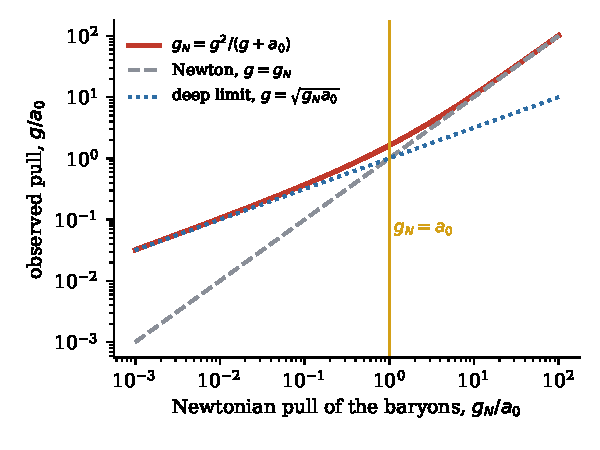
\includegraphics[width=0.85\linewidth]{figures/the_law.pdf}
\caption{The law (red) between its two limits: Newton at high acceleration (grey dashed) and $\sqrt{\gbar a_0}$ at low acceleration (blue dotted). The bend happens at $\gbar\approx a_0$, the only scale in the problem.}
\end{figure}

Equivalently, in Milgrom's notation $g\,\mu(g/a_0)=\gbar$, the law uses
\begin{equation}
\mu(x)=\frac{x}{1+x},
\end{equation}
the ``simple'' interpolating function, which Famaey and Binney found to fit the Milky Way well in 2005.

\fig{interp_family}{The shape knob nobody counts. Four interpolating functions with the same two limits differ by up to 0.1\,dex near the transition. Choosing the simple form is a decision made once; counted honestly, it's a meta-knob.}


\section{Whose idea is it?}

Let me be completely clear about credit, because this book would be worthless if it weren't.
\begin{itemize}
\item The relation between $g$ and $\gbar$, with a single acceleration scale, is \textbf{Milgrom's} modified Newtonian dynamics, proposed in 1983. The simple form of the interpolating function is well known in the MOND literature.
\item The nearness of $a_0$ to $cH_0$ and to $c^2\sqrt\Lambda$ is also \textbf{Milgrom's} observation, from his first papers and again in 1999.
\item The proposal that the scale is tied to the \textbf{dark energy density} was made by \textbf{Limbach, Psaltis and \"Ozel} in 2008.
\end{itemize}
What this programme adds is a particular coefficient, $\kappa=\tfrac12$, which is fitted; a reconstruction of how the scale should change over cosmic time from raw expansion data (Chapter~13); a graded comparison with every rival I could think of (Part~II); and a public record of every failure (Chapter~12).

\section{The numbers}

Using $\rhoDE=5.84\times10^{-27}\,\mathrm{kg\,m^{-3}}$, which corresponds to the dark energy share and expansion rate of the standard reading of the expansion history,
\begin{equation}
a_0=\tfrac12\,c\sqrt{G\rhoDE}=\tfrac12\,(3.00\times10^8)\sqrt{3.90\times10^{-37}}=9.36\times10^{-11}\ms,
\end{equation}
since $G\rhoDE=(6.674\times10^{-11})(5.84\times10^{-27})=3.90\times10^{-37}\,\mathrm{s^{-2}}$.

A few worked examples from the law's limits:
\begin{center}
\begin{tabular}{lrr}
\toprule
baryonic mass & flat speed $v_f=(GMa_0)^{1/4}$ & $r_M=\sqrt{GM/a_0}$\\
\midrule
$10^9\Msun$ (a dwarf) & $59\kms$ & 1.2 kpc\\
$10^{10}\Msun$ & $106\kms$ & 3.9 kpc\\
$6\times10^{10}\Msun$ (Milky Way-ish) & $165\kms$ & 9.4 kpc\\
$10^{11}\Msun$ & $188\kms$ & 12.2 kpc\\
\bottomrule
\end{tabular}

\smallskip
{\footnotesize $r_M$ is the radius at which a point mass's Newtonian pull falls to $a_0$. Real discs are extended, so treat it as a scale, not a boundary. Speeds are on the canonical footing.}
\end{center}

\section{Two footings, never pooled}

There's a subtlety that every honest report of this law has to carry. ``The dark energy density'' and ``the critical density'' differ by the factor $\Omega_\Lambda\approx0.685$, and the programme has always reported results on both readings. They're called \emph{footings}.

\textbf{Canonical footing.} $\kappa=\tfrac12$ on the dark energy density: $a_0=9.3603\times10^{-11}\ms$.

\textbf{Alternative footing.} $\kappa=\tfrac12$ on the critical density $\rho_c=3H_0^2/8\pi G$:
\begin{gather}
a_0=\frac12\,c\sqrt{G\rho_c}=\frac12\,c\sqrt{\frac{3H_0^2}{8\pi}}=\frac{cH_0}{2\sqrt{8\pi/3}}\equiv\frac{cH_0}{Z},\\
Z=2\sqrt{\frac{8\pi}{3}}=5.7888.
\end{gather}
With $H_0=67.4\kms\,\mathrm{Mpc}^{-1}$ this is $1.1312\times10^{-10}\ms$. This was the programme's earliest form, $a_0=cH_0/Z$, before the tie to dark energy was made explicit.

The two values differ by $1/\sqrt{\Omega_\Lambda}\approx1.21$, about $0.08\dex$. Every result is reported on both footings and they're never averaged, because averaging would hide whichever one fails. They differ in a deeper way too: the canonical footing tracks dark energy, so it stays nearly flat in redshift, while the alternative tracks the critical density and rises with $H(z)$. That's the contrast at the heart of Chapter~13.

\section{The knob is fitted}

Now the confession that every chapter after this one depends on. \textbf{$\kappa=\tfrac12$ is not derived.}

The programme's record lists about 550 attempts to derive or select it: from horizon thermodynamics, from entropy arguments, from field equations, from symmetry. None succeeded. A closure analysis (the lane called KC1) reduced every route to the same missing piece. Setting $\kappa=\tfrac12$ is mathematically the same as asserting that some physical length is exactly $c/\sqrt{G\rho}$, and no field equation on record supplies that length. A screen of sixteen further premises found none that does (KC2). Another lane (KF1) found routes that give $\tfrac12$, 1.447 or 1.772 depending on which length you choose, and only the length with no field equation behind it gives $\tfrac12$.

So it's a knob. One knob. I set it.

\section{Does the data even pick \texorpdfstring{$\tfrac12$}{1/2}?}

Not decisively. Here's the profile likelihood over 175 SPARC galaxies, which asks how much worse the fit gets as $a_0$ is moved away from its best value (with galaxy-to-galaxy correlations included in the error estimate):

\begin{center}\small
\begin{tabular}{@{}lrrr@{}}
\toprule
choice of $a_0$ & value ($\ms$) & $\Delta\chi^2$ & significance\\
\midrule
free best fit & $1.0766\times10^{-10}$ & 0 & --\\
$\kappa=\tfrac12$ on $\rhoDE$ (canonical) & $9.36\times10^{-11}$ & 63.90 & 1.82$\sigma$\\
$\kappa=\tfrac12$ on $\rho_c$ (alternative) & $1.1312\times10^{-10}$ & 7.04 & 0.60$\sigma$\\
Milgrom's $cH_0/2\pi$ & $1.042\times10^{-10}$ & 5.34 & 0.53$\sigma$\\
\bottomrule
\end{tabular}
\end{center}

\fig{footings}{Candidate values of $a_0$ on SPARC, with their distance from the free best fit in clustered standard deviations. Milgrom's $cH_0/2\pi$ and the alternative footing sit closer to the best fit than the canonical $\kappa=\frac12$; a $2\pi$ horizon form on $\rho_{\rm DE}$ sits furthest.}

\begin{honestbox}[Milgrom's value fits at least as well]
On SPARC alone, Milgrom's own $cH_0/2\pi$ fits at least as well as my canonical $\tfrac12$, and the alternative footing sits between. The data can't settle the coefficient yet. To tell $\tfrac12$ from $0.461$, the value a $2\pi$ horizon form gives on the dark energy footing, at three standard deviations, you'd need $a_0$ to 2.8 per cent. The shared galaxy-mass floor, the uncertainty that every galaxy shares through stellar mass-to-light ratios and distances, is about 9.5 per cent, and the best case with the dark energy density is about 5 per cent. More archive data won't fix this; only new observations will. And Chapter~8 showed that plausible systematic corrections move the fitted scale by up to $\pm0.15\dex$.
\end{honestbox}

So why $\tfrac12$ at all? Because it's simple, because it puts the scale on the dark energy density with no $\pi$s floating around, and because it was the programme's starting hypothesis. Those are reasons to \emph{choose} it, not evidence that it's right. What makes the choice interesting is what it commits the law to, and that's Part~V.

\section{The honest knob count}

The cleanest way to finish this chapter is with the same knob accounting I applied to everyone else.

\begin{knobbox}{The law's control panel}
\begin{tabular}{@{}lp{6cm}@{}}
\toprule
item & status\\
\midrule
$\kappa$ & \textbf{1 global knob}, fitted; 6.6 bits\\
the scale $\rhoDE$ & not a knob: measured by the expansion of the universe, independently of galaxies\\
the function $\mu(x)=x/(1+x)$ & a shape choice made once (the simple MOND form); counted as a meta-knob\\
per-galaxy $\Upsilon$, distance, inclination & nuisance knobs, paid by \emph{every} theory including \LCDM; fixed at 0.5 and 0.7 in the fried chicken comparison\\
a Solar System screen & needed; the action adopted for it (v3s, Chapter~11) brings its own structure, and $a_0$ still enters it by hand\\
clusters, CMB & \textbf{not covered}; no knob offered (Chapter~12)\\
\bottomrule
\end{tabular}
\end{knobbox}

That last row matters. A theory with one knob that explains only galaxies isn't comparable, knob for knob, with a theory with six knobs that explains the CMB. What the one knob \emph{does} explain, it explains with almost no freedom. Let's see what that buys.
